\documentclass[a4paper,twocolumn]{article}
\usepackage[hmargin={1.1cm,1.1cm},vmargin={2.2cm,2cm}]{geometry}
%       includehead,     scale=0.85,centering,hoffset=-0.1cm,voffset=-0.5cm]{geometry} headheight=13.1pt ,portrait

%\usepackage[a4paper,portrait,twocolumn,includeheadfoot,
%            scale=0.85,centering,hoffset=-1cm]{geometry}
\usepackage[pdftex]{graphicx,color}
\usepackage{amsmath}
\usepackage{amssymb}
\usepackage{stmaryrd}
\usepackage[french]{babel}
\selectlanguage{french}
\usepackage{fancyhdr}
\usepackage{floatflt}
\usepackage{ucs}
\usepackage[utf8]{inputenc}
\usepackage[T1]{fontenc}
\usepackage[pdftex,colorlinks={true},urlcolor={blue},pdfauthor={remy Nicolai}]{hyperref}
\usepackage{makeidx}


%Options de hyperref pour les fichiers pdf g{\'e}n{\'e}r{\'e}s
%\hypersetup{pdfpagemode=None,colorlinks=true,pdffitwindow=true}
%\hypersetup{pdfpagemode=None,colorlinks=true}


%                 Chargement des symboles de l'AMS
%\input amssym
%pour que la compilation aille au bout
%\nofiles\scrollmode

%pr{\'e}sentation du compteur de niveau 2 dans les listes
\makeatletter
\renewcommand{\labelenumii}{\theenumii.}
\makeatother

%dimension des pages, en-t{\^e}te et bas de page
  %utilisation avec vmargin
   %\setpapersize{custom}{21cm}{29.7cm}
   %\setmarginsrb{1.5cm}{0cm}{3.5cm}{1cm}{15mm}{10mm}{0mm}{0mm}
%\setlength{\voffset}{-2cm}
%\setlength{\oddsidemargin}{-1cm}
%\setlength{\textheight}{25cm}
%\setlength{\textwidth}{17.3cm}
%\columnsep=5pt
% \columnseprule=0.5pt
%\columnseprule=0.5pt
%En tete et pied de page
\pagestyle{fancy}
\lhead{Lycée Hoche MPSI B}
%\rhead{}
%\rhead{25/11/05}
\lfoot{\tiny{Cette création est mise à disposition selon le Contrat\\ Paternité-Partage des Conditions Initiales à l'Identique 2.0 France\\ disponible en ligne http://creativecommons.org/licenses/by-sa/2.0/fr/
} }
\rfoot{\tiny{Rémy Nicolai \jobname pdf du \today}}

%\pagestyle{fancy}
%\lhead{MPSI B}
%\rhead{\today}
%\rfoot{\small{\jobname}}
\newcommand{\baseurl}{http://back.maquisdoc.net/data/}
\newcommand{\textesurl}{http://back.maquisdoc.net/data/devoirs_nicolair/}
\newcommand{\exosurl}{http://back.maquisdoc.net/data/exos_nicolair/}
\newcommand{\coursurl}{http://back.maquisdoc.net/data/cours_nicolair/}

\newcommand{\N}{\mathbb{N}}
\newcommand{\Z}{\mathbb{Z}}
\newcommand{\C}{\mathbb{C}}
\newcommand{\R}{\mathbb{R}}
\newcommand{\K}{\mathbf{K}}
\newcommand{\Q}{\mathbb{Q}}
\newcommand{\F}{\mathbf{F}}
\newcommand{\U}{\mathbb{U}}
\newcommand{\p}{\mathbb{P}}


\newcommand{\card}{\mathop{\mathrm{Card}}}
\newcommand{\Id}{\mathop{\mathrm{Id}}}
\newcommand{\Ker}{\mathop{\mathrm{Ker}}}
\newcommand{\Vect}{\mathop{\mathrm{Vect}}}
\newcommand{\cotg}{\mathop{\mathrm{cotan}}}
\newcommand{\cotan}{\mathop{\mathrm{cotan}}}
\newcommand{\sh}{\mathop{\mathrm{sh}}}
\newcommand{\ch}{\mathop{\mathrm{ch}}}
\newcommand{\argch}{\mathop{\mathrm{argch}}}
\newcommand{\argsh}{\mathop{\mathrm{argsh}}}
\newcommand{\tr}{\mathop{\mathrm{tr}}}
\newcommand{\rg}{\mathop{\mathrm{rg}}}
\newcommand{\rang}{\mathop{\mathrm{rg}}}
\newcommand{\val}{\mathop{\mathrm{val}}}

\newcommand{\Mat}{\mathop{\mathrm{Mat}}}
\newcommand{\MatB}[2]{\mathop{\mathrm{Mat}}_{\mathcal{#1}}\left( #2\right) }
\newcommand{\MatBB}[3]{\mathop{\mathrm{Mat}}_{\mathcal{#1} \mathcal{#2}}\left( #3\right) }

\renewcommand{\Re}{\mathop{\mathrm{Re}}}
\newcommand{\Ima}{\mathop{\mathrm{Im}}}
\renewcommand{\Im}{\mathop{\mathrm{Im}}}
\renewcommand{\th}{\mathop{\mathrm{th}}}
\newcommand{\repere}{$(O,\overrightarrow{i},\overrightarrow{j},\overrightarrow{k})$ }
\newcommand{\trans}{\mathstrut^t\!}
\newcommand{\cov}{\mathop{\mathrm{Cov}}}
\newcommand{\orth}[1]{#1^{\perp}}

\newcommand{\absolue}[1]{\left| #1 \right|}
\newcommand{\fonc}[5]{#1 : \begin{cases}#2 &\rightarrow #3 \\ #4 &\mapsto #5 \end{cases}}
\newcommand{\depar}[2]{\dfrac{\partial #1}{\partial #2}}
\newcommand{\norme}[1]{\left\| #1 \right\|}
\newcommand{\se}{\geq}
\newcommand{\ie}{\leq}
\newcommand{\serie}[1]{\left( \sum {#1}_n \right)_{n\in\N}}

\batchmode
 
\begin{document} 
\chead{ Fonctions d’une Variable Géométrique : calcul intégral: énoncés.}
\begin{enumerate}
  \item \begin{tiny}Eig01\end{tiny}
Calculer l'aire comprise entre les deux boucles de la courbe donnée en coordonn{\'e}es polaires par $\rho=2\cos \theta -1$ ( lima\c{c}on de Pascal).
 
  \item \begin{tiny}Eig02\end{tiny}
Calculer les int{\'e}grales curvilignes
  $\int_{\Gamma}\omega$ dans les cas suivants.

\begin{enumerate}
  \item $\omega=x^2dx+y^2dy$, $\Gamma$ est la demi-ellipse
  parcourue dans le sens indirect et d{\'e}finie par
  \[\left \{ \begin{array}{c}
    x^2+4y^2-4=0 \\
    y \geq 0 \
  \end{array} \right.  \]
  \item $\omega=\frac{x-y}{x^2+y^2}dx+\frac{x+y}{x^2+y^2}dy$, $\Gamma$ est
  le contour du carr{\'e} $A,B,C,D$ avec $A=(1,1)$, $B=(-1,1)$,
  $C=(-1,-1)$, $D=(1,-1)$.
  \item $\omega=ydx+2xdy$, $\Gamma$ est le contour, parcouru dans
  le sens direct du domaine d{\'e}fini par
  \begin{displaymath}
\left \{ \begin{array}{c}
    x^2+y^2-2x \leq 0 \\
    x^2+y^2-2y \leq 0 \
  \end{array} \right. 
\end{displaymath}
  \item $\omega=ydx+xdy$, $\Gamma$ est l'arc de parabole $y=x^2$
  parcourue de $O(0,0)$ vers $A(2,4)$.
\end{enumerate} 
  \item \begin{tiny}(Eig03)\end{tiny}
Calculer $\int_D f dx\wedge dy$ dans les cas suivants (on donne $D$
  {\`a} gauche et $f$ {\`a} droite)
\begin{align*}
  D=[0,\pi]^2  & & (x+y)\sin x \sin y \\
  x\geq 0, x^2+y^2\leq 1 & & \frac{y}{x^2+1}\\
  x^4+y^4+x^2-y^2\leq 1 & & 2x(x^2+y)\\
  \frac{x^2}{a^2}+\frac{y^2}{b^2}\leq 1 & & x^2+y^2\\
\end{align*}
 
  \item \begin{tiny}Eig04\end{tiny}
Calculer $\int_D f dxdy$ dans les cas suivants {\`a} l'aide d'un changement de variable.
    \begin{enumerate}
        \item $D$ est limit{\'e} par deux paraboles donn{\'e}es par les in{\'e}quations
            \[y^2-2px\leq 0\quad,\quad    x^2-2py \leq 0\\\]
            $f=\exp\frac{x^3+y^3}{xy}$, utiliser le changement de
            variable $x=u^2v,y=uv^2$.
        \item Soit $a$ et $b$ tels que $0<a<b$, le domaine $D$ est
        d{\'e}fini par les {\'e}quations
        \[a\leq xy \leq b,\quad 0\leq x \leq y,\quad y^2-x^2\leq 1\]
        $f=(y^2-x^2)(x^2+y^2)$, utiliser le changement de variable
        $u=xy,v=y^2-x^2$.\newline
Les fonctions $u$ et $v$ sont définies dans le premier quart de plan.
        \item $D$ est la partie du plan $y>0$ limit{\'e} par les quatre paraboles
        \begin{eqnarray*}
            P_1:y^2=4x+4,\quad P_2:y^2=2x+1\\
            P_3:y^2=9-6x,\quad P_4:y^2=-4x+4\\
        \end{eqnarray*}
        $f=\frac{y}{\sqrt{x^2+y^2}}$, utiliser le changement de variable $x=u^2-v^2,y=2uv$.
    \end{enumerate}
 
  \item \begin{tiny}Eig05\end{tiny}
Montrer que
  \[\forall x \in [0,1], \ln(1+x)=\int_{0}^{1}\frac{x}{1+xy}dy\]
  En d{\'e}duire la valeur de
  \[\int_{0}^{1}\frac{\ln(1+x)}{1+x^2}dx\]
  puis celle de
  \[\int_{0}^{1}\frac{\arctan x}{1+x}dx\] 
  \item \begin{tiny}Eig06\end{tiny}
Soit $D$ le domaine du plan défini par les inégalités :
\begin{displaymath}
  x\geq 0,y\geq 0, x+y\leq 1
\end{displaymath}
Soit $f$ une fonction $\mathcal C^1(\R)$, calculer
\begin{displaymath}
 \int_D f(x+y)dx\wedge dy
\end{displaymath}
en utilisant une primitive $F$ de $f$ et une 1-forme. Appliquer au cas où
$ f(t)=\ln (1+t) $.
 
  \item \begin{tiny}Eig07\end{tiny}
Soit $a$ un réel strictement positif, la ligne de niveau $o$ de la fonction
\begin{displaymath}
 f=x^3+y^3-3axy
\end{displaymath}
est appelée \emph{folium de Descartes}. Elle forme une boucle dans le domaine du plan $x>0$, $y>0$. Dessiner cette boucle et calculer son aire. 
  \item \begin{tiny}Eig08\end{tiny} Intégrale de Dirichlet.\newline
\begin{figure}[h!]
 \centering
 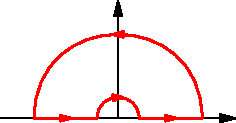
\includegraphics{./Eig08_1.pdf}
 % Eig08_1.pdf: 113x59 pixel, 72dpi, 3.99x2.08 cm, bb=0 0 113 59
 \caption{Exercice \arabic{enumi}}
 \label{fig:Eig08_1}
\end{figure}
Soit $\mathcal{D}$ l'ensemble des points $m$ d'un plan rapporté à un repère tels que $|x(m)|+y(m)>0$. On définit les fonctions $A$ et $B$ par
\begin{align*}
 &A= \frac{e^{-y}}{x^2+y^2}\left( x\sin x - y\cos x\right) \\
 &B= \frac{e^{-y}}{x^2+y^2}\left( x\cos x + y\sin x\right)
\end{align*}
On note $\omega = Adx +Bdy$ et
\begin{displaymath}
 I(r) = \int_0^\pi e^{-r\sin \theta}\cos(r\cos\theta)d\theta
\end{displaymath}
et on admet que $I \xrightarrow{+\infty}0$ et $I \xrightarrow{0}\pi$.
\begin{enumerate}
 \item Dessiner le domaine $\mathcal{D}$. Est-il étoilé ?
 \item Calculer $\frac{\partial A}{\partial y}$ et $\frac{\partial B}{\partial x}$.
 \item Montrer que l'intégrale curviligne de $\omega$ le long de la courbe constituée de segments et de demi-cercles (de rayon $0<r<R$ (figure \ref{fig:Eig08_1}) est nulle.
 \item En exprimant cette intégrale curviligne d'une autre manière montrer que, quand $r\rightarrow 0$,
\begin{displaymath}
 \int_r^{\frac{1}{r}}\frac{\sin t}{t}dt \rightarrow \frac{\pi}{2}
\end{displaymath}

\end{enumerate}
 
\end{enumerate} 
\clearpage 
\chead{Fonctions d’une Variable Géométrique : calcul intégral: corrigés.}
\begin{enumerate}
  \item Cig01.tex manque. 
  \item Cig02.tex manque. 
  \item Cig03.tex manque. 
  \item Cig04.tex manque. 
  \item Cig05.tex manque. 
  \item Cig06.tex manque. 
  \item Cig07.tex manque. 
  \item Cig08.tex manque. 
\end{enumerate} 
\end{document}